\section{Grappa} \label{sec:grappa}

\begin{figure}[t]
\begin{center}
  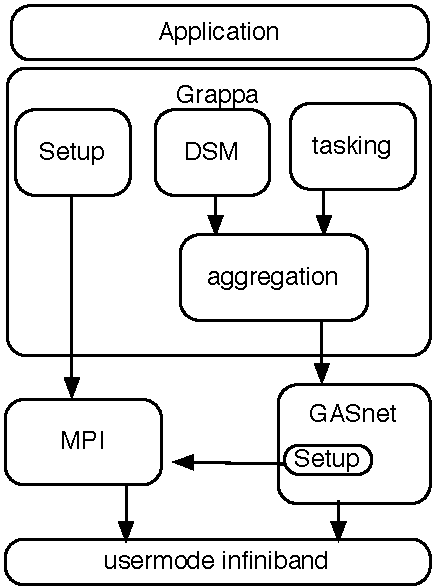
\includegraphics[width=0.5\columnwidth]{figs/grappa-crappy}
\begin{minipage}{0.95\columnwidth}
  \caption{\label{fig:grappa} Grappa runtime system \vspace{-4ex}}
\end{minipage}
\vspace{-3ex}
\end{center}
\end{figure}

In this section we describe the Grappa runtime system
(Figure~\ref{fig:grappa}). Grappa is a software runtime system that
allows a commodity distributed-memory HPC cluster to be programmed as
if it were a single large shared-memory machine. Grappa is designed to
smooth over some of the performance discontinuities in commodity
hardware, giving good performance when there is little locality to be
exploited while allowing the programmer to exploit it when it is
available.

Grappa provides three key capabilities. The first is a distributed
shared \textbf{global memory} with high aggregate random access
bandwidth. The second is a \textbf{tasking} system with lightweight
multithreading and automatic load balancing through work
stealing. Finally, under the hood, a \textbf{communication} layer uses
network packet scheduling and aggregation to achieve high performance
while remaining largely invisible to applications.

In the following sections, we discuss the programmer's view of
Grappa's main capabilities, including a subset of the Grappa API. In
section~\ref{implementation}, we discuss the details of their
implementation.


\subsection{Tasks}

%The basic unit of locality in Grappa is the {\em core}. Each core is
%responsible for a section of the global memory

The basic unit of execution in Grappa is the {\em task}. Tasks are
small; just a function pointer and some arguments. Tasks are only
queued when they are spawned; later, when resources are free, they are
allocated a stack, bound to a core, and executed.

What makes Grappa's tasks special is that when they perform
long-latency operations they can give up control of their core,
allowing the core to remain busy while waiting for the operation to
complete. This most often done implicitly inside a call into Grappa's
API, but it can also be done explicitly by the programmer using the
calls shown in Figure~\ref{fig:scheduling}. \TODO{cite UPC split phase
    reads and writes, but include that we provide a way to overlap
    computation}

All Grappa scheduling is done in userspace, and minimal state is
saved, in order to minimize the context switch time. In our
experiments, we saw context switch times as low as \TODO{40ns}.

This lightweight context switching is Grappa's key enabling
feature. It gives us the ability to tolerate latency. Given that
ability, we are able to trade latency for throughput: by {\em
  increasing} latency in key components in the system we are able to
increase our aggregate random access bandwidth, our synchronization
bandwidth, and our ability to tolerate load.

\begin{figure}[htbp]
  \begin{center}
    \begin{description}\small
    \item[ \texttt{ yield() } ] \hfill \\
      Gives up control of core to scheduler, queuing task to be scheduled again soon
    \item[ \texttt{ suspend() } ] \hfill \\
      Gives up control of core to scheduler
    \item[ \texttt{ wake( task * $t$ ) } ] \hfill \\
      Enqueues $t$ to be scheduled again soon
    \end{description}
    \begin{minipage}{0.95\columnwidth}
      \caption{\label{fig:scheduling} Grappa API: scheduling} %{-4ex}}
    \end{minipage}
    %\vspace{-3ex}
  \end{center}
\end{figure}


\subsection{Expressing parallelism}

A programmer's goal in coding with Grappa should be to express as much
parallelism as possible without worrying about where it will execute.
Grappa then chooses where and when to execute this parallelism,
scheduling as much work as necessary to tolerate network latencies and
keep the systems' cores busy. 

Grappa provides four methods for expressing parallelism, shown in
Figure~\ref{fig:expressing-parallelism}. The first is explicit task
spawns. When the programmer identifies work that can be done in
parallel, the work may be wrapped up in a function and queued with its
arguments for later execution using a \texttt{spawn}. Sometimes the
programmer may want to spawn a task on a specific core in the system,
or at the home core of a particular memory location. Grappa provides a
\texttt{spawn\_on} call for this purpose; the task is immediately
enqueued on the specified core and is not available to other cores.

The next method for expressing parallelism is a parallel for loop,
where the number of iterations must be known at loop entry. The programmer specifies
a function pointer along with start and end indices and an optional
threshold to control parallel overhead. Grappa does {\em recursive decomposition} of iterations,
 as in the implementation of Cilk's cilk\_for construct \TODO{cite cilk\_for implementation:
     could only find slides page6 of http://www.clear.rice.edu/comp422/lecture-notes/comp422-2012-Lecture5-Cilk++.pdf}.
It generates a logarithmically-deep tree of tasks, stopping to execute
the loop body when the number of iterations is below the threshold (``grainsize'' in Cilk).
\TODO{we may want to make our classification purer: the for loop is
    not Grappa's core, and is built atop tasks as a useful construct; in some sense the only way
to express parallelism in Grappa is tasks and perhaps call\_on. -BM}

Finally, a programmer may want to run a small piece of code on a
particular core in the system without waiting for execution resources
to be available. Grappa provides the \texttt{call\_on} call for this
purpose.

\begin{figure}[htbp]
  \begin{center}
    \begin{description}\small
    \item[ \texttt{spawn( void (*fp)(args) )} ] \hfill \\
      Creates a new stealable task
    \item[ \texttt{spawn\_on( core, (*fp)(args) )} ] \hfill \\
      Creates a new private task that will run on a specific core 
    \item[ \texttt{parallel\_for( (*fp)(args), start, end )} ] \hfill \\
      Executes iterations of a loop as stealable tasks 
    \item[ \texttt{call\_on( core, (*fp)(args) )} ] \hfill \\ 
      Runs a limited function on a specific core without consuming
      Grappa execution resources 
    \end{description}
    \begin{minipage}{0.95\columnwidth}
      \caption{\label{fig:expressing-parallelism} Grappa API: expressing parallelism} % \vspace{-4ex}}
    \end{minipage}
    %\vspace{-3ex}
  \end{center}
\end{figure}

\subsection{Accessing memory}

Applications written for Grappa utilize two forms of memory: local and
global.

Local memory is local to a single core in the system.  Accesses occur
through conventional pointers.  The compiler emits an access and the
memory is manipulated directly.  Applications use local accesses for a
number of things in Grappa: the stack associated with a task, accesses
to localized global memory in caches (see below), and accesses to
debugging infrastructure that is local to each system node.  Local
pointers cannot access memory on other cores, and are valid only on
their home core.

Large data that is expected to be accessed with low locality is stored in Grappa's global memory. All
global data must be accessed through calls into Grappa's API, shown in
Figure~\ref{fig:accessing-memory}.

Grappa provides two methods for {\emph storing} data in the global memory. The
first is a distributed heap striped across all the machines in the
system. The \texttt{global\_malloc} and \texttt{global\_free} calls
are used to allocate and deallocate memory in the global heap; on
allocation, a global pointer is returned. Grappa also allows any local
data on a core's stacks or heap to be exported to the global address
space to be made accessible to other cores across the system.

There are also two approaches to {\emph accessing} global memory. When the
programmer expects a computation on shared data to have spatial
locality to exploit, {\em cache} operations may be used. When there is no locality to
exploit, {\em delegate} operations are used. Since these operations
are expected communicate with other nodes and have high latency,
\TODO{...}

With a cache, applications can instruct Grappa to fetch a global
pointer of any length and return a local pointer to a cached copy of
the global memory. Under the hood, Grappa performs the mechanics of
gathering chunks of data from multiple system nodes and presenting a
conventional appearing linear block of memory as a pointer into a
cache. Grappa cache operations have the usual read-only and read-write
variants, along with a write-only variant used to initialize data
structures. Cache operations exploit spatial locality by reducing the number of small network
messages accessing contguous data. Languages for distributed
shared memory systems have done optimizations to achieve a similar goal. The UPC compiler
coalesces struct and array accesses into 
remote get/put \cite{Chen:2005}, or Fortran D compiler's message
vectorization that hoists small messages out of a loop
\cite{FortranD:1992}. Caching in Grappa additionally provides a
mechanism for exploiting temporal locality by operating on the data locally. 

When the access pattern has low-locality, it is more efficient
to modify the data on its home core rather than bringing a copy to the
requesting core and returning it after modification. Delegate
operations provide this capability. Applications can dispatch
computation to be performed on individual machine-word sized chunks of
global memory to the memory system itself (e.g.,
\emph{fetch-and-add}).

Delegate operations, proposed in \cite{Nelson:hotpar11}, are also the primary synchronization method in
Grappa. Each piece of global memory is paired with a single core in
the system; all accesses to that memory are done by that core. This
allows delegate operations to be performed atomically on the core
simply by making sure no other code interleaves; since context
switches in Grappa are cooperative, this is trivial. Thus, delegate
operations are able to provide atomic semantics to memory owned by one core without using atomic
operations. Using delegation to implement isolation for any subset of
memory has been explored in \cite{delegated:oopsla11}.

\begin{figure}[htbp]
  \begin{center}
    \begin{description}\small
      \item[ \texttt{ global\_address global\_malloc( size )} ] \hfill \\
      \item[ \texttt{ global\_free( global\_address )} ] \hfill \\
        Allocates and frees memory in the global heap
      \item[ \texttt{ delegate\_read( global\_address, local\_var )} ] 
      \item[ \texttt{ delegate\_write( global\_address, local\_var )} ] \vspace{-2ex}
      \item[ \texttt{ delegate\_cas( global\_address, local\_var )} ] \vspace{-2ex}
      \item[ \texttt{ delegate\_inc( global\_address, local\_var )} ] \vspace{-2ex} \hfill \\
        Performs a memory operation at the home core of a global address
      \item[ \texttt{ cache\_acquire( global\_address, local\_buf, \{RO,RW,WO\})} ]
      \item[ \texttt{ cache\_release( global\_address, local\_buf )} ] \vspace{-2ex} \hfill \\
        Perform cache operations \TODO{expand}
    \end{description}
    \begin{minipage}{0.95\columnwidth}
      \caption{\label{fig:accessing-memory} Grappa API: accessing memory} %{-4ex}}
    \end{minipage}
    %\vspace{-3ex}
  \end{center}
\end{figure}



\subsection{Under the hood}

Grappa contains two key components that are not directly visible to
the programmer but are key to providing good performance. Both depend
on Grappa's ability to tolerate latency in order to obtain this
performance.

The first is a dynamic load balancing mechanism that uses work stealing to
move tasks from busy nodes to idle nodes. When a core detects that it
has idle execution resources and no new tasks to run, it issues steal
requests over the network. The core continues to execute remaining
active work while the steal requests are in flight. When a steal
request succeeds, it returns with more tasks that can be matched with
execution resources and scheduled.

The second is a network packet scheduling and aggregation system. From
the perspective of the application, all communication between tasks in
Grappa takes place either through global shared memory or remote task
spawns. Both of these requests are ultimately translated into explicit
inter-system-node/core communication requests that are dispatched to
the \gasnet~library. Most of \checkme{our requests} are small, and commodity
networks do not transport small packets efficiently. In order to make
more efficient use of bandwidth, Grappa aggregates packets going to the
same destination until it can form a larger packet that will make more
efficient use of the network. In this way, Grappa trades per-request
latency for application-level throughput.
